\section{Математические модели}
    <<Ресурс>> в реальных экосистемах можно разделить на два вида:
    \begin{itemize}
        \item Энергия, например, солнечный свет. Тогда экосистема с данным ресурсом является незамкнутой, и энергия <<протекает>> через систему, в ходе этого рассеиваясь в виде тепла.
        \item Биологические вещества, например, углерод, азот, фосфор. В этом случае экосистема является замкнутой по отношению к ресурсам. Достигается это деятельностью так называемых <<разлагателей>>, которые разлагают мёртвую органику до необходимых минеральных компонентов, необходимых первичным уровням трофической цепи.
    \end{itemize}

    Соответственно будем рассматривать два типа трофической цепей: незамкнутые (<<проточные>>) и замкнутые (<<циклы>>).

    Рост и развитие экосистем во многих системах лимитируется каким-либо фактором (\textit{принцип Либаха}). Опять же, например, солнечный свет -- это невозобновимый ресурс и цепь является незамкнутой, а химические вещества за счёт разлагателей снова вовлекаются в деятельность замкнутой экосистемы.
    
    \begin{figure}[H]
    \centering
    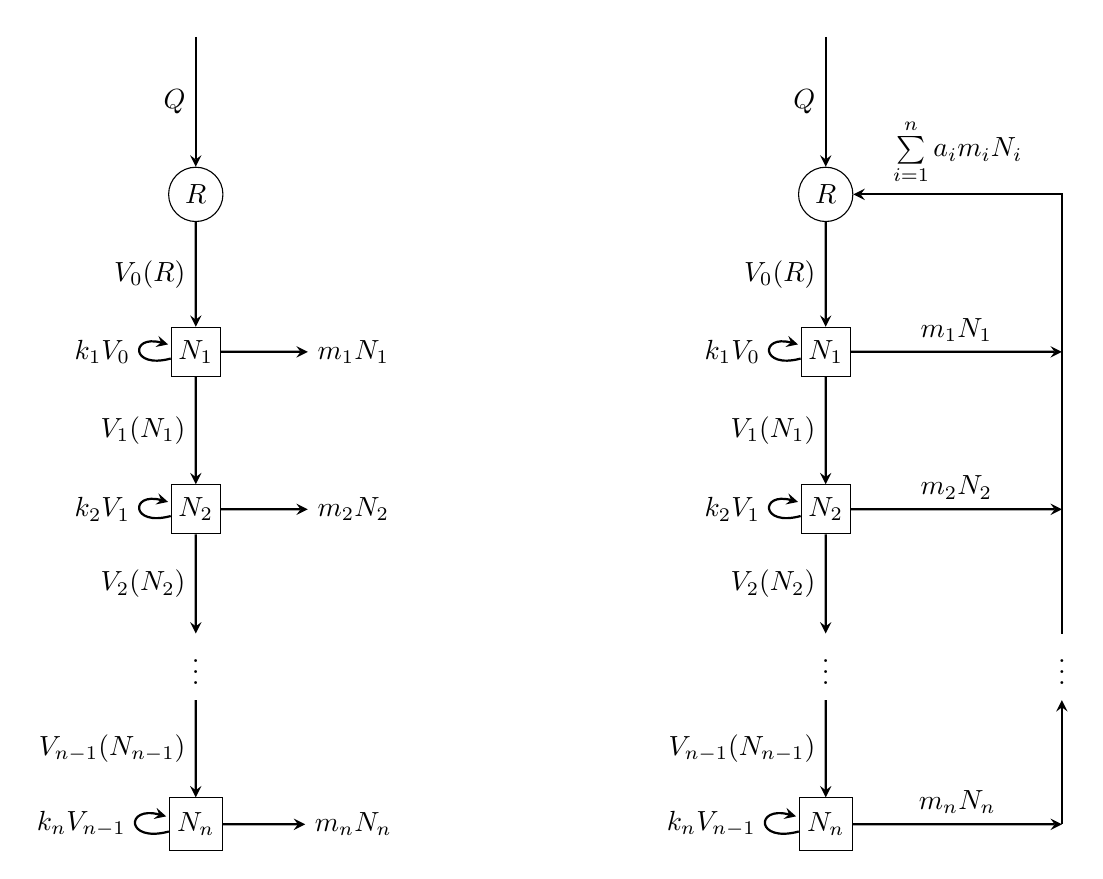
\begin{tikzpicture}

        \usetikzlibrary{shapes.geometric, calc}

        \tikzstyle{roundnode} = [draw, circle, text centered];
        \tikzstyle{squarenode} = [draw, regular polygon, regular polygon sides=4, text centered, inner sep=0];
        \tikzstyle{arrow} = [thick, ->, >=stealth];
    
        % Left - Flow
        \node[roundnode] (RF) at (0,8) {$R$};

        \node[squarenode] (NF1) at (0,6) {$N_1$};
        \node (NF1M) at (2,6) {$m_1 N_1$};
        \draw [arrow] (NF1) -- (NF1M);

        \node[squarenode] (NF2) at (0,4) {$N_2$};
        \node (NF2M) at (2,4) {$m_2 N_2$};
        \draw [arrow] (NF2) -- (NF2M);

        \node (DF) at (0,2) {$\vdots\vphantom{lp}$};

        \node[squarenode] (NFN) at (0,0) {$N_n$};
        \node (NFNM) at (2,0) {$m_n N_n$};
        \draw [arrow] (NFN) -- (NFNM);


        \draw [arrow] (0,10) -- node[anchor=east] {$Q$} (RF);
        \draw [arrow] (RF) --   node[anchor=east] {$V_0(R)$} (NF1);
        \draw [arrow] (NF1) --  node[anchor=east] {$V_1(N_1)$} (NF2);
        \draw [arrow] (NF2) --  node[anchor=east] {$V_2(N_2)$} (DF);
        \draw [arrow] (DF) --   node[anchor=east] {$V_{n-1}(N_{n-1})$} (NFN);


        \path[arrow] (NF1) edge [loop left] node {$k_1 V_0$} ();
        \path[arrow] (NF2) edge [loop left] node {$k_2 V_1$} ();
        \path[arrow] (NFN) edge [loop left] node {$k_n V_{n-1}$} ();
        % Left - Flow
        
        % Right - Cycle
        \node (BTC) at (11, 10) {};
        \node (BBC) at (11, 0) {};

        \node[roundnode] (RC) at (8,8) {$R$};

        \node[squarenode] (NC1) at (8,6) {$N_1$};
        \draw [arrow] (NC1) -- node[anchor=south] {$m_1 N_1$} ($(BTC)!(NC1)!(BBC)$);

        \node[squarenode] (NC2) at (8,4) {$N_2$};
        \draw [arrow] (NC2) -- node[anchor=south] {$m_2 N_2$} ($(BTC)!(NC2)!(BBC)$);

        \node (DC) at (8,2) {$\vdots\vphantom{lp}$};
        \node (DC2) at ($(BTC)!(DC)!(BBC)$) {$\vdots\vphantom{lp}$};

        \node[squarenode] (NCN) at (8,0) {$N_n$};
        \draw [arrow] (NCN) -- node[anchor=south] {$m_n N_n$} ($(BTC)!(NCN)!(BBC)$);


        \draw [arrow] (8,10) -- node[anchor=east] {$Q$} (RC);
        \draw [arrow] (RC) --   node[anchor=east] {$V_0(R)$} (NC1);
        \draw [arrow] (NC1) --  node[anchor=east] {$V_1(N_1)$} (NC2);
        \draw [arrow] (NC2) --  node[anchor=east] {$V_2(N_2)$} (DC);
        \draw [arrow] (DC) --   node[anchor=east] {$V_{n-1}(N_{n-1})$} (NCN);
        
        \draw [arrow] (DC2) |- node[pos=0.75, anchor=south] 
        {$\textstyle\sum\limits_{i=1}^n a_i m_i N_i$} (RC);


        \path[arrow] (NC1) edge [loop left] node {$k_1 V_0$} ();
        \path[arrow] (NC2) edge [loop left] node {$k_2 V_1$} ();
        \path[arrow] (NCN) edge [loop left] node (KNVN1) {$k_n V_{n-1}$} ();

        \draw [arrow] ($(KNVN1)!(BTC)!(NCN)$) -- (DC2);
        % Right - Cycle

    \end{tikzpicture}
    \caption{CAPTION}
    \end{figure}


    \pagebreak
    Вот такой вид диффура моделей.

    \begin{equation} \label{flow}
        Q -> N_i
    \end{equation}


    \begin{equation} \label{cycle}
        Q -> N_i -> Q + a_i * N_i
    \end{equation}

    Исследуем равновесия и их устойчивость при изменении параметра \(Q\).

    \subsection{Тут ещё}
        Долги вывод и всё такое.

    \begin{figure}[H]
        \centering
        % 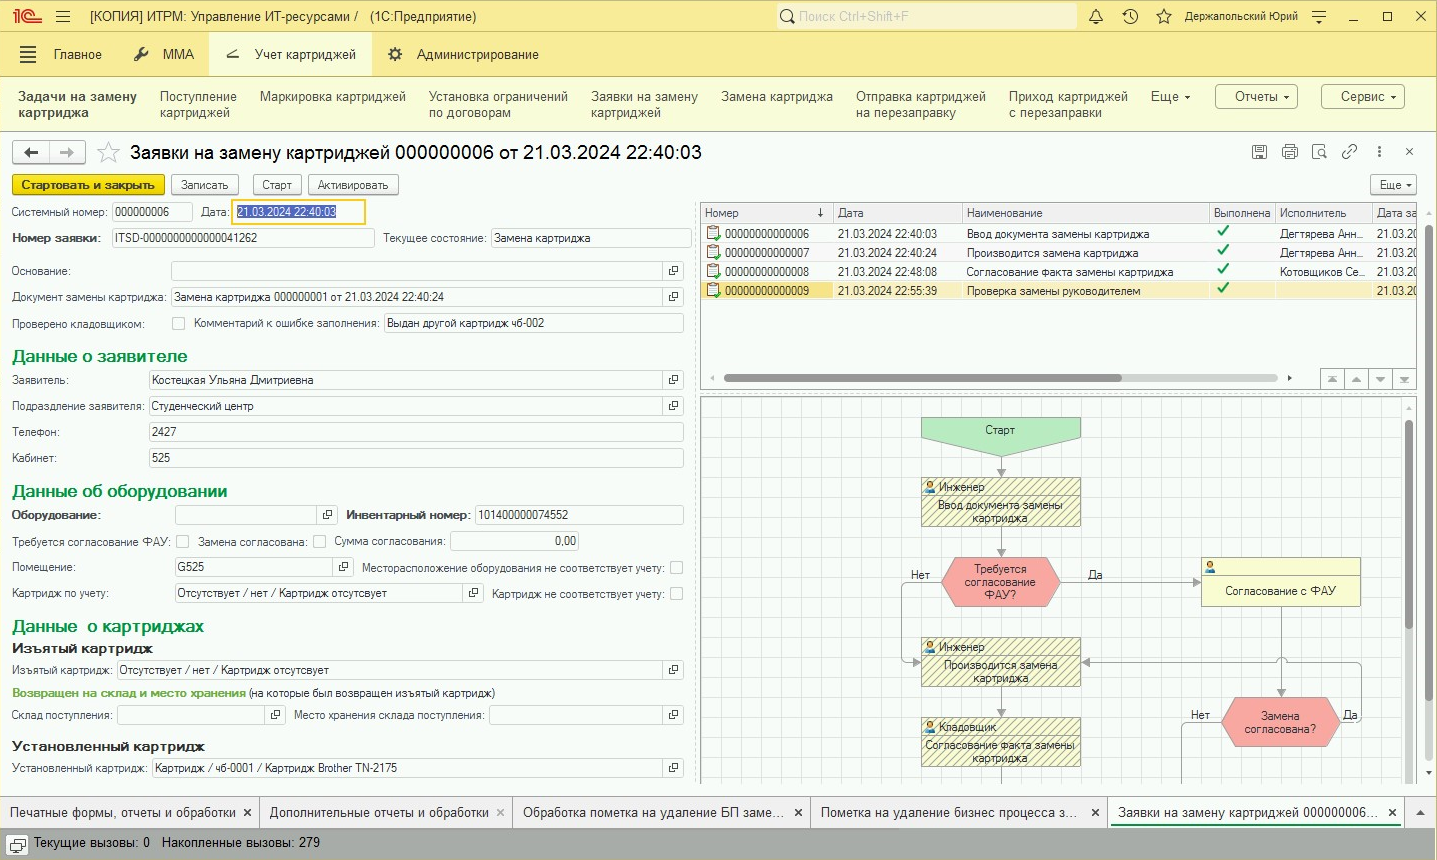
\includegraphics[width=14cm]{pictures/process.png}
        \caption{}  \label{pic_label}
    \end{figure}

